\documentclass[tikz]{standalone}

\usepackage{tikz}
\usetikzlibrary{calc}
\usetikzlibrary{arrows.meta}

\begin{document}
    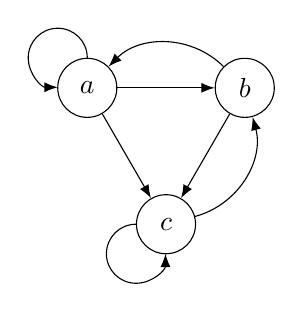
\begin{tikzpicture}[
        remember picture,
        every node/.style={draw,circle,minimum size=0.75cm,inner sep=-1pt},
        >=Latex
    ]
        \node (a) at (0,0) {$a$};
        \node (b) at ($(a) + (0:2)$) {$b$};
        \node (c) at ($(a) + (-60:2)$) {$c$};
        \draw[->] (a) -- (b);
        \draw[->] (a) -- (c);
        \draw[->] (b) -- (c);
        \path[->] (b) edge[bend right=45] (a);
        \path[->] (c) edge[bend right=45] (b);
        \draw[->] (a.north) arc(0:270:0.375);
        \draw[->] (c.west) arc(90:360:0.375);
    \end{tikzpicture}
\end{document}